%%% LaTeX Template: Designer's CV
%%%
%%% Source: http://www.howtotex.com/
%%% Feel free to distribute this template, but please keep the referal to HowToTeX.com.
%%% Date: March 2012


%%%%%%%%%%%%%%%%%%%%%%%%%%%%%%%%%%%%%
% Document properties and packages
%%%%%%%%%%%%%%%%%%%%%%%%%%%%%%%%%%%%%
\documentclass[a4paper,11pt,final]{memoir}

% misc
\renewcommand{\familydefault}{bch}	% font
\pagestyle{empty}					% no pagenumbering
\setlength{\parindent}{0pt}			% no paragraph indentation

\newcommand\tab[1][1,8cm]{\hspace*{#1}}

% required packages (add your own)
\usepackage{flowfram}										% column layout
\usepackage[top=1cm,left=0.5cm,right=0.5cm,bottom=0.5cm]{geometry}% margins
\usepackage{graphicx}										% figures
\usepackage{url}											% URLs
\usepackage[usenames,dvipsnames]{xcolor}					% color
\usepackage{multicol}										% columns env.
	\setlength{\multicolsep}{0pt}
\usepackage{paralist}										% compact lists
\usepackage{tikz}
\usepackage[utf8]{inputenc}
%%%%%%%%%%%%%%%%%%%%%%%%%%%%%%%%%%%%%
% Create column layout
%%%%%%%%%%%%%%%%%%%%%%%%%%%%%%%%%%%%%
% define length commands
\setlength{\vcolumnsep}{\baselineskip}
\setlength{\columnsep}{\vcolumnsep}

% frame setup (flowfram package)
% left frame
\newflowframe{0.22\textwidth}{\textheight}{0pt}{0pt}[left]
	\newlength{\LeftMainSep}
	\setlength{\LeftMainSep}{0.2\textwidth}
	\addtolength{\LeftMainSep}{1\columnsep}
 
% small static frame for the vertical line
\newstaticframe{1.5pt}{\textheight}{\LeftMainSep}{0pt}
 
% content of the static frame
\begin{staticcontents}{1}
\hfill
\tikz{%
	\draw[loosely dotted,color=RoyalBlue,line width=1.5pt,yshift=0]
	(0,0) -- (0,\textheight);}%
\hfill\mbox{}
\end{staticcontents}
 
% right frame
\addtolength{\LeftMainSep}{1.5pt}
\addtolength{\LeftMainSep}{1\columnsep}
\newflowframe{0.7\textwidth}{\textheight}{\LeftMainSep}{0pt}[main01]


%%%%%%%%%%%%%%%%%%%%%%%%%%%%%%%%%%%%%
% define macros (for convience)
%%%%%%%%%%%%%%%%%%%%%%%%%%%%%%%%%%%%%
\newcommand{\Sep}{\vspace{1.5em}}
\newcommand{\SmallSep}{\vspace{0.2em}}

\newenvironment{AboutMe}
	{\ignorespaces\textbf{\color{RoyalBlue} About me}}
	{\Sep\ignorespacesafterend}
	
\newcommand{\CVSection}[1]
	{\Large\textbf{#1}\par
	\normalsize\normalfont}

\newcommand{\CVItem}[1]
	{\textbf{\color{RoyalBlue} #1}}


%%%%%%%%%%%%%%%%%%%%%%%%%%%%%%%%%%%%%
% Begin document
%%%%%%%%%%%%%%%%%%%%%%%%%%%%%%%%%%%%%
\begin{document}

% Left frame
%%%%%%%%%%%%%%%%%%%%
\begin{figure}
	\hfill
	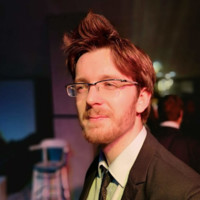
\includegraphics[width=0.6\columnwidth]{photo}
	\vspace{-7cm}
\end{figure}

\begin{flushright}\small
	LACOUR Florian \\
	\url{florlacour@gmail.com}  \\
	06 12 22 54 91
\end{flushright}\normalsize
\framebreak


% Right frame
%%%%%%%%%%%%%%%%%%%%
\Huge\bfseries {\color{RoyalBlue}  LACOUR Florian} \\
\Large\bfseries  Ingénieur Informatique \\ \\
% Education
\CVSection{Education}
\CVItem{2012  - 2017,UTBM }\\
Université de Technologie de Belfort Montbéliard (90) Ingénieur en Informatique Logiciel Embarqué et Temps réel 

% Experience
\CVSection{Experiences}

\CVItem{Janvier 2018, Capgemini (Lille) }\\
\textbf{Auchan}: EFOOD: site E-Commerce\\
\tab ECOMM: Site ROPO (Research Online Purchase Offline)\\
\tab PHOENIX:  Initialisation d'un site E-commerce avec des technologies micro-services\\
\textbf{Taches  }   \textbullet  Développement de la partie editoriel du site \\
\tab \textbullet  Participation à l'équipe DevOps avec pour objectif la réduction du time to market \\
\tab \textbullet Maintenance du run (You build it you run it) \\
\tab \textbullet Participation à l'élaboration d'une architecture micro-service  \\
 \textit{Technologie utilisé}: JAVA (Spring, SpringBoot, JSP, SPRING MVC, Hibernate), Javascript/HTML/CSS, Junit/Mockito, Docker, Maven/Ant, Git / GitlabCi / Jenkins, Linux, Ansible, Sonar, Methode Agile/Devops, ReactivePrograming, micro-services, ReactJs/VueJs, SAP Hybris

\CVItem{Septembre 2017-Janvier 2018, Thales Services (Paris) }\\
\textbf{CIRUS}: Automatisation de la livraisons d'applications\\
 \textit{Technologie utilisé}: Ansible, Terraform, Python, Git, GitlabCi, Methode Agile \\
 \textbf{FACEBOT}: Detection automatique de visages sur des photos/videos que cella soit en mobilité (Android) ou sur un poste \\
 \textit{Technologie utilisé}: Android (JNI), Python (Flask), C++ (Dlib), Neo4J, Git 


\CVItem{Février-Juillet 2017, Parkeon (Besançon)}\\
\textbf{AFCANDEV}: Création d’une application de maintenance pour des validateurs de ticket de métro. \\
 \textit{Technologie utilisé}: Android(Java), ReactJs, Junit, Jenkins, Python, Git, methode agile


% Skills
\CVSection{Skills}
\CVItem{Développement applicatif}
\begin{multicols}{2}
\begin{compactitem}[\color{RoyalBlue}$\circ$]
	\item Java: Spring/Hibernate/Spring Cloud
	\item  JUnit/Mockito/Expresso/Robolectric
	\item  HTML5/CSS,  ReactJS, Vue.js
	\item Android
	 \item Kotlin 
	\item C++
\end{compactitem}
\end{multicols}

\CVItem{Outils }
\begin{multicols}{3}
\begin{compactitem}[\color{RoyalBlue}$\circ$]
	\item Jenkins/GitlabCi
	\item  Docker/Rancher/Swarm
	\item  Ansible/ Terraform
\end{compactitem}
\end{multicols}
\CVItem{Methods}
\begin{multicols}{2}
\begin{compactitem}[\color{RoyalBlue}$\circ$]
	\item Agile (Kamban, SCRUM)
	\item  Devops
\end{compactitem}
\end{multicols}


\begin{minipage}{0.30\textwidth}
\CVSection{Langue }
\begin{enumerate}[\color{RoyalBlue}$\circ$]
  \item Anglais courant (C1-BULAT)\\

\end{enumerate}
\end{minipage}%
\hfill
\begin{minipage}{0.63\textwidth}
\SmallSep
\CVSection{Hobbies}
\begin{tabular}{|p{\textwidth}}
\begin{multicols}{1}
\begin{enumerate}[\color{RoyalBlue}$\circ$]
  \item Animateur en colonies de vacance 
  \item Music (Trompette/Trombone)   
\item Triathlon
\end{enumerate}
\end{multicols}
\end{tabular}
\end{minipage}%
\framebreak



%%%%%%%%%%%%%%%%%%%%%%%%%%%%%%%%%%%%%
% End document
%%%%%%%%%%%%%%%%%%%%%%%%%%%%%%%%%%%%%
\end{document}